\section{Smart Card Simulator}

The Smart Card Simulator is a tool to generate transaction codes (also referred to as TANs), implemented in Java. This tool is available for download to users who choose SCS as the preferred way to received TANs, at the time of their registration with the Bank. The SCS relies mainly on the PIN, that is sent to the user through an e-mail after registration is approved by an employee.
The SCS is not personalized i.e., it is not unique based on the user. Also, there
are no hard-coded passwords or tokens for user identification stored anywhere in
the JAR. This is a good thing as an attacker cannot get hold of any user-specific
information by just getting access to the SCS. \\

Once the SCS has been downloaded by the user, it can be used to generate TANs. The SCS works in two modes thereby supporting Single Transaction and Batch Transactions respectively.
\begin{itemize}
\item Single Transaction: The SCS takes 3 inputs - Account ID of the Recipient, Amount to be transferred and the PIN for the SCS. 
\item Batch Transactions: The SCS takes only 2 inputs - Batch file containing the transaction details in the prescribed format and the PIN for the SCS.
\end{itemize}
Refer figure \ref{fig:scs_modes} for the view of the Smart Card Simulator. \\

The SCS generates the TAN after performing basic validations such as entry of mandatory fields and format of inputs. Validations such as existent recipient, valid pin, sufficient balance etc. are handled at the PHP end at the time of actual transfer. \\

Java code is organized mainly in 2 classes - \code{SmartCardSimulator.java} and \\ \code{TanGenerator.java}. \textbf{SmartCardSimulator} handles the display of the interface and the TAN generation logic is handled by the \textbf{TanGenerator}.
Refer figure \ref{fig:scs_class_diagram} for the complete Class diagram of the Smart Card Simulator.


The TanGenerator removes all white-spaces from the inputs, and concatenates the current time in milliseconds divided by 10 5 (=100 seconds) to the input. This input string is then hashed with the \code{SHA512} hashing
algorithm. The first 15 characters of this hash are the tan number for the corresponding transaction.
The purpose of using the current time is to set an expiration time for the generated TAN. This makes the code unusable after 100 seconds. There is a minor possibility of client and server time not being in sync which could lead to the TAN becoming unusable. \\

The TAN generated by the SCS is used in the online transfer form. 
At the PHP side, a TAN is generated using a similar algorithm as in Java, using
the target and amount entered in the Web UI and the SCS pin of the user fetched
from the database. If the TAN(from SCS) entered by the user matches this TAN,
payment is processed successfully. \\

\begin{figure}[ht]
	\centering
	\begin{subfigure}{.45\textwidth}
		\centering
		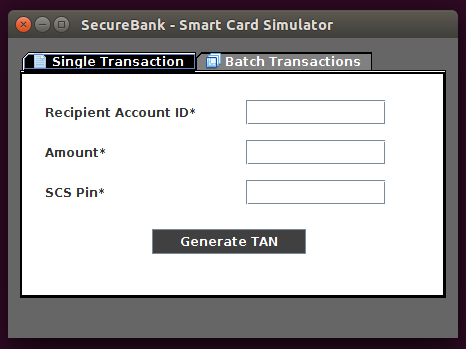
\includegraphics[width=.9\linewidth]{figures/scs_mode_single.png}
		\caption{View for Single Transaction}
	\end{subfigure}\hfill%
	\begin{subfigure}{.45\textwidth}
		\centering
		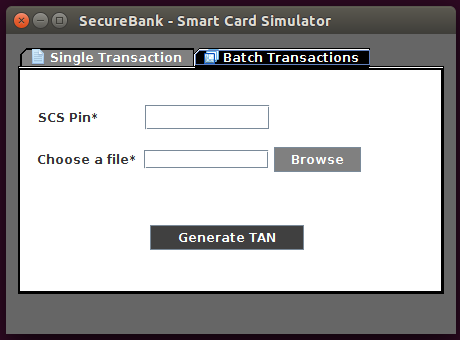
\includegraphics[width=.9\linewidth]{figures/scs_mode_batch.png}
		\caption{View for Batch Transaction}
	\end{subfigure}
	\caption{Smart Card Simulator}
	\label{fig:scs_modes}
\end{figure}


\begin{figure}[ht]
	\centering
	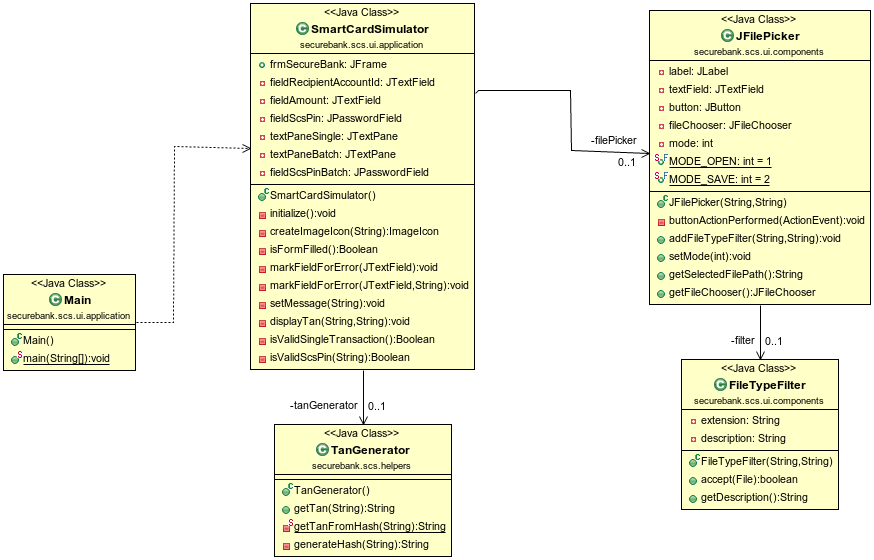
\includegraphics[width=.8\linewidth]{figures/scs_class_diagram.png}
	\caption{Class Diagram of Smart Card Simulator}
	\label{fig:scs_class_diagram}
\end{figure}

\clearpage